\subsection{E-field Lines and Equipotential surfaces}

\subsubsection{a}
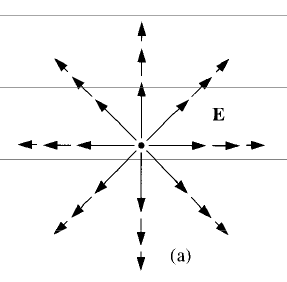
\includegraphics{img/3_1_a}

\subsubsection{b}
The information is the line 'density'.

\subsubsection{c,d}
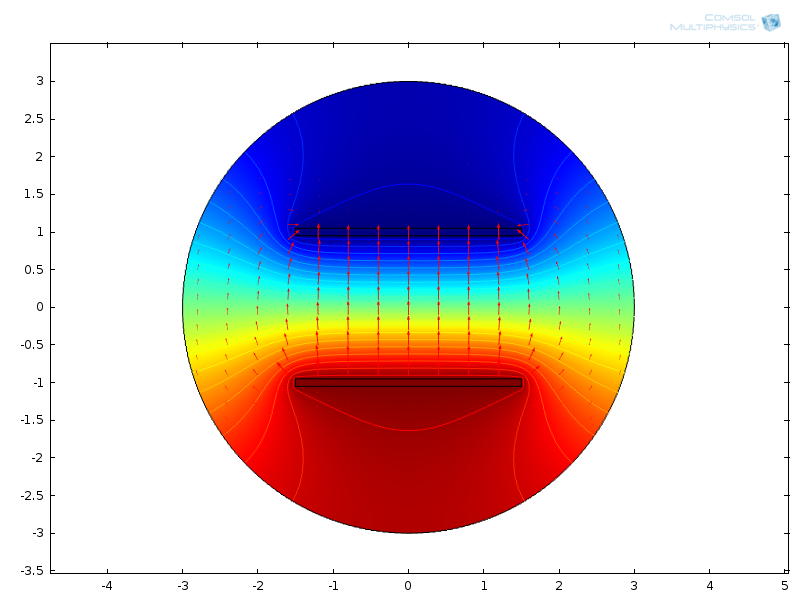
\includegraphics[scale=0.5]{img/3_1_c,d}

\subsubsection{e}
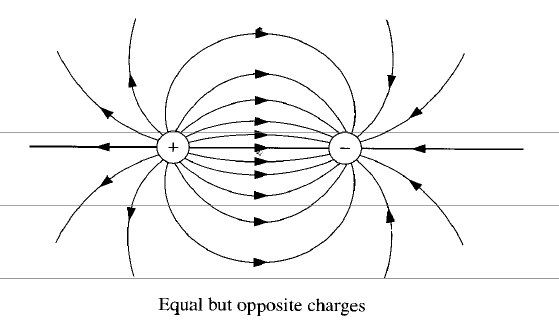
\includegraphics[scale=0.7]{img/3_1_e}
Dipole field/equipotential = see lecture notes.
Like gradient, equipotential lines \(\perp\) to \(\vec{E}\) field.

\subsection{Excercise 2 - Electric field and potential of a straight wire/rod}

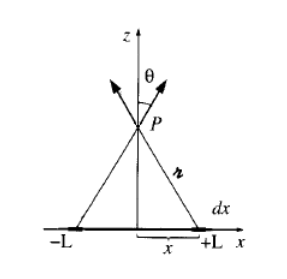
\includegraphics{img/3_2}

\subsubsection{}
Just by looking at the graph, \(x\) terms should cancel by symetry. So we look
for \(y\) terms.

Small segment: \(d\vec{E}_y\)
\[
	d\vec{E}_y =
		\frac{1}{4 \pi \epsilon_0} \frac{dq}{r^2} \cos{\theta} \hat{y}
\]
\[
	dq = \lambda dx
\]
\[
	\cos{\theta} = \frac{z}{r}
\]
\[
	r = \sqrt{x^2+z^2}
\]
By replacing into the main equation, we have
\[
	d\vec{E}_y =
	\frac{1}{4 \pi \epsilon_0} \frac{\lambda dx}{r^2} \frac{z}{r} \hat{y}
\]
By integrating in respect to x, we obtain
\[
	\vec{E}_y =
	\int_{-L}^L \frac{1}{4 \pi \epsilon_0}
	\frac{z \lambda dx}{(\sqrt{x^2+z^2})^2} \hat{y}
\]
By reducing the integral
\[
	\vec{E}_y =
	\frac{\lambda z}{4 \pi \epsilon_0}
	\int_{-L}^L \frac{dx}{(\sqrt{x^2+z^2})^2} \hat{y}
\]
We use the "helper" form
\[
	\vec{E}_y =
	\frac{\lambda z}{4 \pi \epsilon_0}
	\left.\frac{x}{z^2 \sqrt{L^2+z^2}} \hat{y}\right|_{-L}^L
\]
We compute with the two limits
\[
	\vec{E}_y =
	\frac{\lambda L}{2 \pi \epsilon_0 \sqrt{z^2+L^2}} \hat{y}
\]
Now that we have to result, we verifiy it when \(z \gg L\)
\[
	\vec{E}_y \approx
	\frac{\lambda L}{2 \pi \epsilon_0 z^2} \hat{y}
\]
If we take \(Q = \lambda 2 L\)
\[
	\vec{E}_y \approx
	\frac{1}{4 \pi \epsilon_0} \frac{Q}{z^2} \hat{y}
\]
Which is what we wanted to find.

\subsubsection{}
Now we take \(L \gg z\)
\[
	\vec{E}_y \approx
	\frac{\lambda}{2 \pi \epsilon_0 z} \hat{y}
\]
The electric potential would be trivially calculated as
\[
	V = - \int_{\infty}^r E dl
\]
But, as the wire is infinite, our reference will also have infinite energy,
so we take another one, for now, we call it \(x\)
\[
	V = - \int_x^r \frac{\lambda}{2 \pi \epsilon_0 z} dz
	= \frac{\lambda}{2 \pi \epsilon_0} \left. \ln(z) \right |_x^r
\]
To nullify easily one part, we take \(z = 1\)
\[
	V = \frac{\lambda}{2 \pi \epsilon_0} (\ln(r) - \ln(1))
	= \frac{\lambda \ln(r)}{2 \pi \epsilon_0}
\]
For example of another point of reference, the \(220 V\) current in the walls
are counted from the ground reference instead of \(\infty\).

\subsection{Electric field and Potential of a disk}

\subsubsection{}
First, we remark that, by symetry, only there is only a force on the \(z\)
component.
We take a small electric field acting on \(P\)
\[
	\vec{dE} = \frac{1}{4 \pi \epsilon_0} \frac{dq}{r^2} \hat{r}
\]
As there is only an action on \(z\)
\[
	\vec{dE}_z = dE \cos{\theta} \hat{z}
	= \frac{1}{4 \pi \epsilon_0} \frac{dq}{r^2} \cos{\theta} \hat{z}
\]
\[
	\cos{\theta} = \frac{z}{r}
\]
\[
	dq = 2 \pi r dr \sigma
\]
\[
	r = \sqrt{r^2+z^2}
\]
We integrate with respect to r
\[
	\vec{E}_z = \int_0^R \frac{1}{4 \pi \epsilon_0}
		\frac{2 \pi r dr \sigma}{r^2} \frac{z}{r} \hat{z}
	= \frac{z \sigma}{2 \epsilon_0}
	\int_0^R \frac{r dr}{(r^2 + z^2)^{3/2}} \hat{z}
\]
By integration by part, we have
\[
	\vec{E}_z = \frac{z \sigma}{2 \epsilon_0}
	( \left. \frac{-1}{\sqrt{r^2+z^2}} \right |_0^R ) \hat{z}
	= \frac{z \sigma}{2 \epsilon_0}
		( \frac{1}{z} - \frac{-1}{\sqrt{R^2+z^2}} ) \hat{z}
\]

\subsubsection{}

We take \(R \gg z\)
\[
	\sqrt{R^2 + z^2} \approx R
\]
So, we can write
\[
	\vec{E}_z = \frac{z \sigma}{2 \epsilon_0} \frac{1}{z} \hat{z}
	= \frac{\sigma}{2 \epsilon_0} \hat{z}
\]
So, we have
\[
	\begin{array}{l l l}
		1D & \lambda &
		\vec{E}_z = \frac{\lambda}{4 \pi \epsilon_0 z} \hat{z} \\
		2D & \sigma  &
		\vec{E}_z = \frac{\sigma}{2 \epsilon_0} \hat{z}
	\end{array}
\]
// TODO unable to read

\subsubsection{}

If we take \(\infty\) as reference, it will be too big
\[
	V = - \int_{x}^z \frac{\sigma}{2 \epsilon_0} dz
	= \left. \frac{- \sigma}{2 \epsilon_0} \right|_x^z
\]
Let \(x = 0\)
\[
	V = \frac{- \sigma}{2 \epsilon_0} z
\]
Is COMSOL ok? Yes, it is, the potential seems to linearly increase between the
plates

\subsubsection{}

\[
	\vec{E}_z = \frac{z \sigma}{2 \epsilon_0}
	( \frac{1}{z} - \frac{1}{\sqrt{R^2+z^2}} ) \hat{z}
\]
If we take \(z \gg R\), we will get zero, so we use the given substitution
\[
	\frac{1}{\sqrt{1 + x}} \approx 1 - \frac{x}{2} + \frac{3 x^2}{8}
\]
\[
	\frac{1}{\sqrt{R^2+z^2}} = \frac{1}{z} (1 + \frac{R^2}{z^2})^{1/2}
	\approx \frac{1}{z} (1 - \frac{R^2}{2 z^2} + 0)
	\approx \frac{1}{z} (1 - \frac{R^2}{2 z^2})
\]
\[
	\vec{E}_z = \frac{z \sigma}{2 \epsilon_0}
	( \frac{1}{z} - \frac{1}{z}  + \frac{1}{2 z} \frac{R^2}{z^2}) \hat{z}
	= \frac{\sigma R^2}{4 z^2 \epsilon_0} \frac{\pi}{\pi} \hat{r}
\]
If we take \(Q = \pi R^2 \sigma\)
\[
	\vec{E}_z = \frac{1}{4 \pi \epsilon_0} \frac{Q}{2^z} \hat{r}
\]

\subsection{Drilling into a disk}

\subsubsection{}

We think of it as a superposition of a plain disk and addition of a hole
\[
	\vec{E}_z = \frac{z \sigma}{2 \epsilon_0}
	( \frac{1}{z} - \frac{1}{\sqrt{R^2 - z^2}} ) -
	\frac{z \sigma}{2 \epsilon_0}
	( \frac{1}{z} - \frac{1}{\sqrt{R_2^2 - z^2}} )
	= \frac{z \sigma}{2 \epsilon_0}
	( \frac{1}{\sqrt{R_2^2 - z^2}} - \frac{1}{\sqrt{R^2 - z^2}} )
\]

\subsubsection{}
